\documentclass[10pt,twocolumn,letterpaper]{article}

\usepackage{cvpr}
\usepackage{times}
\usepackage{epsfig}
\usepackage{graphicx}
\usepackage{amsmath}
\usepackage{amssymb}

\usepackage{pythonhighlight}

% Include other packages here, before hyperref.

% If you comment hyperref and then uncomment it, you should delete
% egpaper.aux before re-running latex.  (Or just hit 'q' on the first latex
% run, let it finish, and you should be clear).
\usepackage[pagebackref=true,breaklinks=true,letterpaper=true,colorlinks,bookmarks=false]{hyperref}

\cvprfinalcopy % *** Uncomment this line for the final submission

\def\cvprPaperID{****} % *** Enter the CVPR Paper ID here
\def\httilde{\mbox{\tt\raisebox{-.5ex}{\symbol{126}}}}

% Pages are numbered in submission mode, and unnumbered in camera-ready
\ifcvprfinal\pagestyle{empty}\fi
\begin{document}

%%%%%%%%% TITLE
\title{%
  Building Automatic Agendas for AAC using a\\ 
    recommendation system with deep learning models  \\
    [3ex]
  \large Advanced Computer Architectures Project report
}
  
\author{
Angela Remolina\\
Politecnico di Milano\\
{\tt\small angelasofia.remolina@mail.polimi.it}
\and
Sergio Pardo\\
Politecnico di Milano\\
{\tt\small sergio.pardo@mail.polimi.it}
}

\maketitle
%\thispagestyle{empty}

%%%%%%%%% ABSTRACT
\begin{abstract}
This paper explores the development of an automated agenda creation system for Augmentative and Alternative Communication (AAC) using a recommendation system powered by deep learning models. The primary objective is to assist educators in designing personalized schedules for individuals with communication disorders. Utilizing TensorFlow Recommenders, the system employs content-based filtering techniques, allowing educators to input external information and create customized activity schedules tailored to the needs of their students. The recommendation system adapts dynamically through reinforcement learning, continuously refining its suggestions based on user interactions and feedback. This approach not only aims to enhance the effectiveness of AAC tools but also to promote inclusivity by addressing the diverse needs of individuals with communication impairments. The proposed model demonstrates significant potential facilitating better educational tools and developmental outcomes.

\end{abstract}

%%%%%%%%% BODY TEXT
%------------------------------------------------------------------------
\section{Introduction}
Inclusion is a constant topic debated in today's society and represents a challenge in many ways, specially, when it comes to removing the barriers that usually set apart disabled people from our society. No matter the cause, disease, injury or developmental disorders, it is of the utmost importance to keep innovating and trying new ways of overcoming the marginalization of this part of the population. There are many types of disabilities, but this article will mainly focus on the ones related to communication. \\

A communication disorder is an impairment of any of the processes by means of which speakers produce, and hearers comprehend, spoken, written, or signed utterances \cite{Cummings2023}. Given this definition, it is possible to see that there is not a single way in which this condition express itself, aggravated by the fact that the age, socioeconomic, ethnic and racial backgrounds of individuals in this position are widely ranged \cite{AAC}. In other words, a solution that perfectly works for every person with apparently the same problem does not exist. This is where modern computer science can play a significant role by applying a series of models that serve multiple purposes and can be tailored for tasks and users alike. \\

This paper takes the AMBRA (\textit{Pervasive and Personalized
Augmentative and Alternative Communication based on
Federated Learning and Generative AI}), approach \cite{AMBRA} as a basis to keep on exploring the possibility of having an open contribution platform where professionals, working on improving on the tools and living conditions for people with communication disorders, will be able to share their knowledge and the contents created with other educators. The key point to this platform, is that it will integrate several technologies, getting the best publicly available methods of state-of-the-art models for each task, enhancing the process of content creation and the possible adaptability of each solution to a particular case. The AMBRA platform takes as foundation the Augmentative and Alternative Comunication (AAC), or better, it is a new proposed implementation of it.\\
 
Given this background, the creation of agendas are a key point to educators as they play an important role in the life of the students with disabilities. They can help decrease the feeling of anxiety, serve as a tool to develop desired skills on a daily basis and ease the construction of a bedtime routine that is critical for the quality of life \cite{tomato}. \\

This last element in the context of communication disabilities is precisely the scope of this project. Particularly, the creation of visual and customised schedules using the latest deep learning models available in the cloud. The objective is facilitating this process to the educators, making them suggestions of activities that could be useful to a particular individual based on its characteristics and the activities that have been already chosen for them. \\



%------------------------------------------------------------------------


\section{Theoretical framework}
Before the beginning of the study it is needed to clarify each concept that is relevant to the project in matter. Some of these terms and definitions are enumerated in this section.

\subsection{Recommender Systems}
Recommender systems (RS) have become integral to many digital platforms, assisting users by suggesting products, services, or content tailored to their preferences. These systems operate by analyzing user behavior and leveraging data to provide personalized recommendations. Broadly, recommender systems can be categorized into three main types \cite{recommenderSystems}:

\begin{enumerate}

    \item Content-Based Filtering: This approach consists in creating profiles for users and/or products to extract significant qualities that could shine some light on the user's preferences. These profiles are then used to try to find the best match between users and products. External information is often required by this method to be able to build the user's profile, so it is not always an easy method to implement.

    \item Collaborative Filtering: This method predicts a user's preferences based on the preferences of other users. It creates an implicit profile of the user based on previous experiences with other products. A drawback to collaborative filtering is it suffers from \textit{cold start}; the system may have trouble addressing new products or users to the environment since there is no historical information.
    
    The two major sub-areas to collaborative filtering are:

        \textbf{Neighborhood Collaborative Filtering}:
        
        Consists in finding users and items that are close or similar to each other. This means there will be neighborhoods of users and items and they will be related to each other depending on the implementation. Algorithms like k-nearest neighbors (k-NN) are often used in this context. \\


        \textbf{Latent Factor Collaborative Filtering}:
        
        This method aims do discover the dimensions that best describe products and users. You could discover natural dimensions, for example, the genre of a movie, but also some hidden dimensions like the pace of said movie. These dimensions can be compared between products to discover similar products and the users that like them.
        

    \item Hybrid Methods: These combine content-based and collaborative filtering techniques to overcome the limitations of each approach. By integrating multiple data sources and recommendation techniques, hybrid methods aim to provide more accurate and diverse recommendations.
    
\end{enumerate}

\subsection{Reinforcement Learning}
Reinforcement learning (RL) is a type of machine learning where an agent learns to make decisions by performing actions and receiving feedback from its environment. Unlike supervised learning, which requires labeled input-output pairs, RL focuses on learning from the consequences of actions. Key components of reinforcement learning include: 
    
\begin{itemize}

    \item Agent: The decision-maker that interacts with the environment.
    
    \item Environment: The external system the agent interacts with.
    
    \item State: A representation of the current situation of the environment.
    
    \item Action: Choices made by the agent that affect the state.
    
    \item Reward: Feedback from the environment based on the action taken.

    \item Policy: The strategy that the agent employs to determine its actions.

    \item Value Function: Estimates the expected long-term return of states or actions, guiding the agent to make optimal decisions.
        
\end{itemize}



\section{Integration of Recommender Systems and Reinforcement Learning for Personalized Agendas}
Combining recommender systems with reinforcement learning can significantly enhance the personalization of agendas. Here’s how this integration works\cite{RLRS}:

\begin{enumerate}
    
    \item Dynamic Adaptation: Reinforcement learning enables recommender systems to adapt dynamically to user feedback. By continuously learning from user interactions, the system can adjust recommendations in real-time, offering a more personalized experience.

    \item Exploration and Exploitation: Reinforcement learning balances exploration (trying new recommendations) and exploitation (leveraging known user preferences). This balance ensures that the system not only caters to current user preferences but also discovers new interests.

    \item Context-Awareness: With reinforcement learning, recommender systems can incorporate contextual information, such as time of day, location, and user activity patterns, to provide more relevant suggestions.

    \item Long-Term Optimization: Reinforcement learning focuses on long-term rewards, helping to optimize user engagement over time rather than just immediate satisfaction. This approach can improve user retention and satisfaction by aligning recommendations with the user's evolving needs and preferences.
    
\end{enumerate}

These 2 fields of study are of big interest to tech giants, so they keep being researched on and probably new models will come in the next years. \\


Personalized agendas benefit from this integration by providing users with tailored schedules and reminders based on their habits, preferences, and goals. For instance, a personalized agenda system can recommend activities that align with the individual's patterns of behaviour, preferred activities and the activities that help them the most throughout the process. By employing reinforcement learning, the system can refine its recommendations through continuous interaction, ensuring that the agenda evolves with the user.\\

This is the potential that current state-of-the-art models and technology have in helping educators in their mission to make this society a more inclusive one. Although the present implementation does not achieve this extend, it is possible to see through this review that AAC can be enhanced by taking advantage of today's technology and ingenuity.
%------------------------------------------------------------------------



\section{Proposed approach}
Our approach to building a system capable of personalizing agendas based on the context (fixed activities) and the preferences of the user (the educator planning the schedule of his pupil) was based on recommender systems. More specifically it was decided the system would be a content-based filtering, given the fact that educators know the profile of the individual to which they are designing the schedule and have external information they could input into the system, in order to trace to them the most suitable activities. Nonetheless, the most prioritized attribute of the RSs was the learning one; the system will learn on each individual preference's and will try to extrapolate this learning to other individuals with the same characteristics. Hence, the system would be able to provide recommended activities for the schedules of individuals who have never had this type of attention before, boosting the progress of their learning.


\section{Implementation}
\subsection{General system architecture}

The complete system architecture consists of three main components that interact with each other. The workflow can be seen below in figure \ref{fig:architecture}. 

\begin{figure*}
  \frame{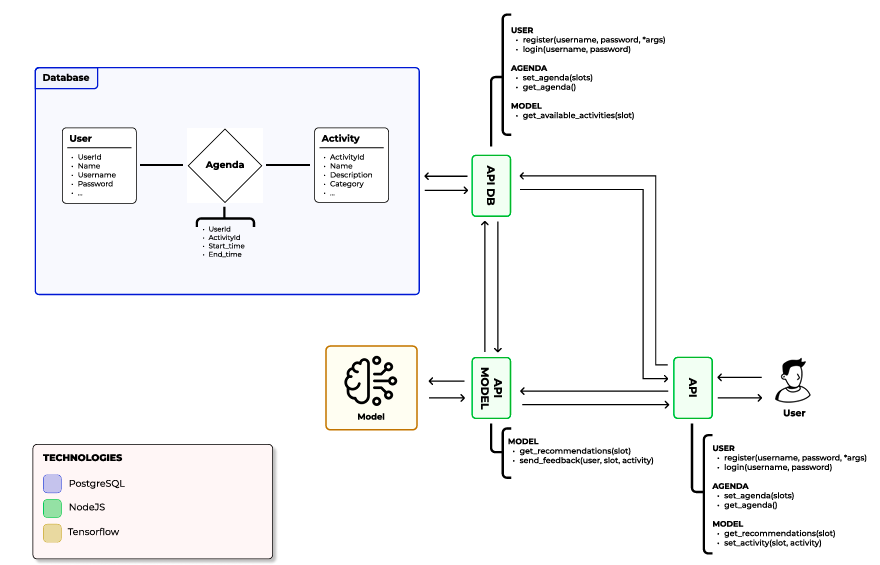
\includegraphics[width=\textwidth]{Diagrams/architecture.png}}
       \centering
       \caption{Proposed architecture for the system.}
       \label{fig:architecture}
\end{figure*}

\begin{enumerate}
    \item \textbf{PostgreSQL Database}: This database stores all the activities and user data. It is accessed via an API that supports CRUD operations (Create, Read, Update, Delete).
    
    \item \textbf{Python Model with TensorFlow}: This model is responsible for generating activity recommendations. It has its own API to receive recommendation requests and user feedback.
    
    \item \textbf{General API in Node.js}: This API serves as the intermediary, connecting user queries to the database and the recommendation model. It handles the communication between the front-end (user requests) and the other components
\end{enumerate}


\subsection{The workflow}
\begin{enumerate}
\item User Query: The user makes a query through the general API in Node.js.
\item Database Interaction: The general API queries the PostgreSQL database to retrieve necessary information about activities and users. E.g. Request to show the agenda for that specific user.
\item Recommendation Generation: The general API requests recommendations from the TensorFlow model in Python.
\item Response to User: The general API sends the generated recommendations back to the user.
\item User Feedback: The user provides feedback on the recommendations, selecting the activity that wants to add to his agenda, which is sent to the general API and then to the Python model to improve future recommendations.
\end{enumerate}
This architecture ensures each component specializes in specific tasks and all interactions are efficiently managed through the APIs.

\subsection{Two-tower retrieval model architecture}
Selecting the architecture of the model is a crucial step in the modeling process of the recommendation system. Since there are two entities the model should have into account: \textbf{User} and \textbf{Activity}, then a two-tower retrieval model is the chosen for the model architecture. Each tower is constructed independently before combining them into the final model. The building is illustrated in the following figure \ref{fig:tower}. 

\begin{figure}[h]
       \frame{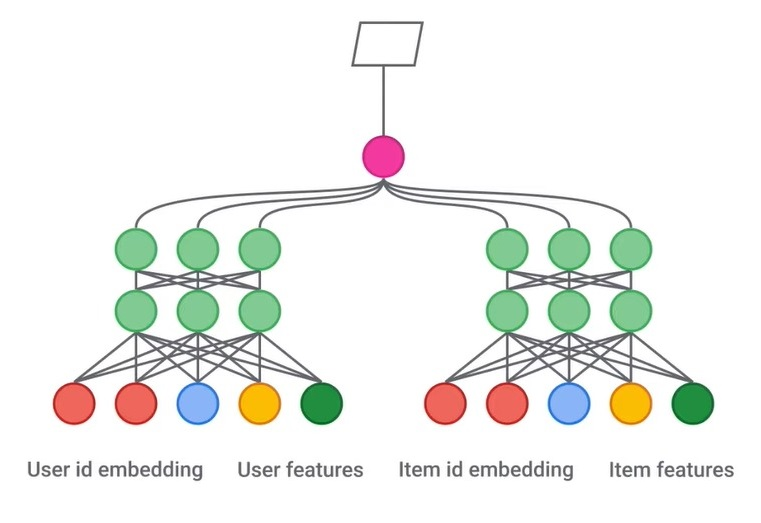
\includegraphics[scale=0.4]{Diagrams/tower_model.jpg}}
       \centering
       \caption{Tower model. Image taken from \cite{tfrs}}
    \label{fig:tower}
\end{figure}

In the context of this project the \textit{item} named above refers to an activity to be recommended e.g. Do yoga, play chess, etc. So \textit{"item id embedding"} refers to the \textbf{Activity ID} embedded into a tensor and  \textit{"item features"} refers to \textbf{Activity features}. The features taken by the model are the name of the activity and its category (sport, boardgame, dancing, etc.). The \textit{"User id emmbeddings"} and \textit{"User features"} represent the corresponding user information and characteristics. 

To model the desired environment, 2 main entities were modeled: the user, meant as the individual to which the schedule is assigned, although the person designing the schedule is the educator. And the Activities that can be included in the schedule. This simple model allows each user to have a set of activities they will be doing based on the days they are assigned to them. 

The activities include the following attributes:

\begin{itemize}

    \item \textbf{id}: unique activity identifier

    \item \textbf{title}: name of the activity

    \item \textbf{category}: An assigned category that adds value to the recommender system's search.

    \item \textbf{description}: Description of the activity itself.

    \item \textbf{start\_time}: Date and time at which the activity starts (which can be chosen by the educator)

    \item \textbf{end\_time}: Date and time at which the assigned activity will end (coherent with \textbf{start\_time})

    \item \textbf{always\_open}: indicates if the activity is free of time restrictions.

    \item \textbf{image}: visual representation of the name of the activity.
    
\end{itemize}

Whereas the user's attributes are the following:

\begin{itemize}

    \item \textbf{id}: unique user identifier

    \item \textbf{name}: complete name of the user (the person using the agenda).

    \item \textbf{username}: unique username for the user in the system.

    \item \textbf{email}: unique email for the user.

    \item \textbf{hashed\_password}: a codified version of the users password to be verified during the login process.
    
\end{itemize}


%-------------------------------------------------------------------------





\section{System prototype}

A prototype of the proposed system was developed to demonstrate its functionality. The system architecture includes a PostgreSQL database with a CRUD API, a recommendation model built using TensorFlow in Python, and a general API in Node.js that integrates user queries, database interactions, and the recommendation model.  Additionally, a simple frontend was created using Handlebars to visualize the system better. It is important to note that this is a low-fidelity prototype, and more sophisticated designs can be implemented to enhance the user experience. See figure \ref{fig:prototype}

\begin{figure*}
  \frame{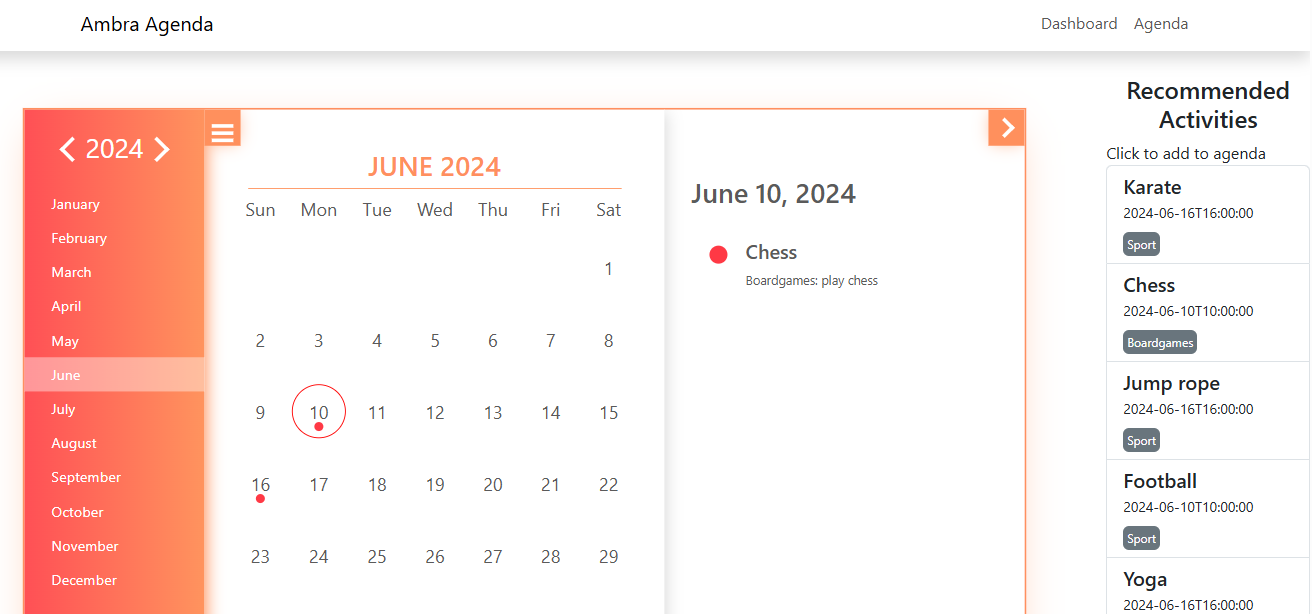
\includegraphics[width=\textwidth]{Diagrams/Agenda-prototype.png}}
       \caption{Prototype for the proposed system.}
       \label{fig:prototype}
\end{figure*}


\section{Conclusions and future work} 

A glimpse into the world of communication disabilities was taken. Afterwards, some of the possibilities that modern techniques and algorithms offer to AAC were tackled on this paper, focusing personalized schedules via the recommendation of activities for people with communication problems, either permanent or ambulatory. Consequently, a possible implementation with tools available for free on the cloud, particularly tensorflow, was developed to show an initial prototype for a potential system to be. As it was said previously, this system takes as foundation the content-base filtering of Recommender Systems, therefore, the extension of the system with a collaborative filtering part could improve it, specially in finding neighbour users, that tend to exhibit the same patterns. As also said in section 2, the fusion with reinforcement learning can improve the performance of the system in the long run.

%-------------------------------------------------------------------------
\appendix

\section{Supplementary Material} 
The source code for this project can be found at https://github.com/AngelaRemolina/AutomaticAgenda-AMBRA

%-------------------------------------------------------------------------



{
\bibliographystyle{ieee}
\bibliography{egbib}
}

\end{document}
